\section{Conclusiones y trabajo futuro }

\begin{frame}[t]{System overview}
	\frametitle{\secname}
	\vspace{-0.5cm}
	\begin{tikzpicture}[remember picture, overlay]
	\node<1->[anchor = north west, text width =0.8\textwidth, yshift = -0.75cm](txt) at (current page.north west) {
		\begin{tcolorbox}[enhanced,title =\secname,width=\textwidth]
		\begin{itemize}
		\item<1-> Se logran obtener excelentes resultados para su publicaci\'on
		\item<2-> Se establece una plataforma de estudio para experimentos futuros
		\item<3-> Se logro abrir camino a la realizacion de herramientas y codigos numericos mediante la creacion de un repositorio en GitHub, donde se comparten para su mejora continua.
		\end{itemize}
		\end{tcolorbox}	
	};


	\node<2->[anchor=south west,inner sep=0mm,xshift=0mm,yshift=0mm] at (current page.south west){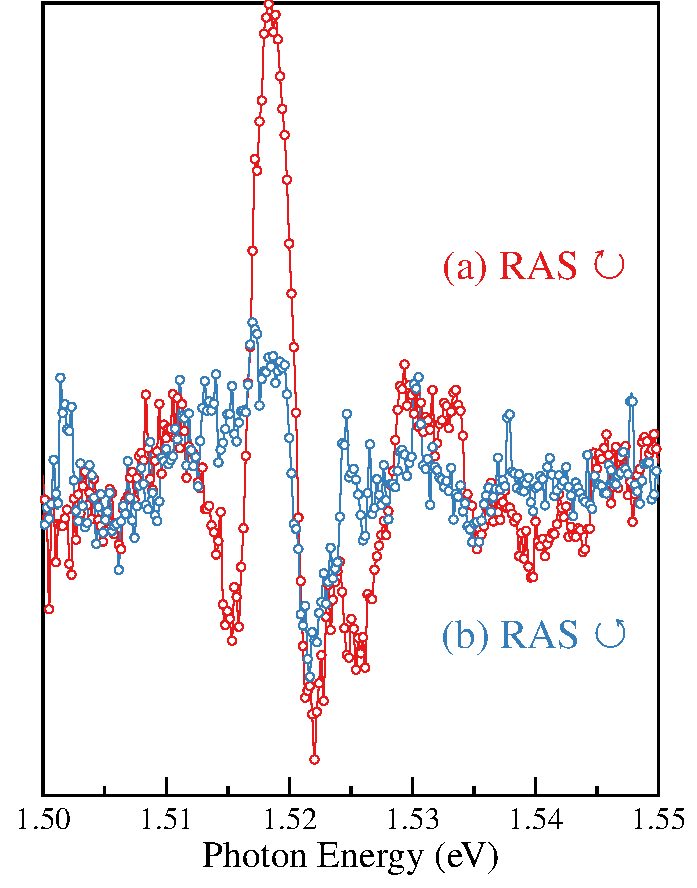
\includegraphics[width=0.42\textwidth]{../../figures/chapter-4/ras-spin/out/ras-spin-1.pdf}};

	\node<3->[anchor=north west,inner sep=0mm,xshift=1mm,yshift=0mm](g1) at (txt.south){
\includegraphics[width=0.6\textwidth]{../beamer-figures/conclusions/git1}};
	\node<3->[anchor=north,inner sep=0mm,xshift=0mm,yshift=0mm] at (g1.south){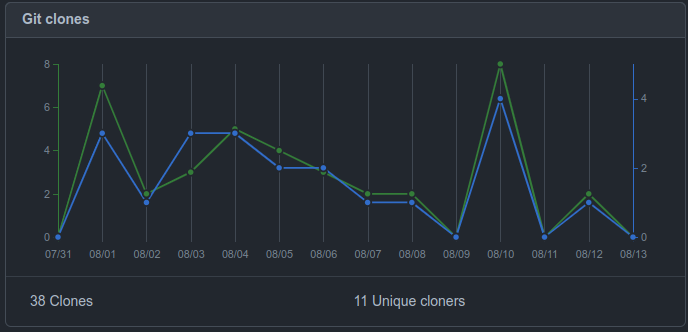
\includegraphics[width=0.6\textwidth]{../beamer-figures/conclusions/git2}};
	
	\end{tikzpicture}
	\end{frame}